\section{Retransmission Based Grouping ACB}
    \label{proposed}
    In this section, we introduce a new grouping concept of ACB and describe it how to dynamically set the ACB factor according to the congestion level.


    To the best of our knowledge, the eNB will broadcasts the information about random access before MTC devices perform the random access procedure. In addition, we let the eNB broadcasts an additional message which is used to group MTC devices into several groups.  We suppose the MTC devices will be classified into two groups, so the eNB will broadcast two kinds of messages for these two groups. Moreover, the contents in the new message are the range of the number of preamble transmissions. As shown in Fig.~\ref{fig_broadcast_groups}
    \begin{figure}[t]
    \centering
    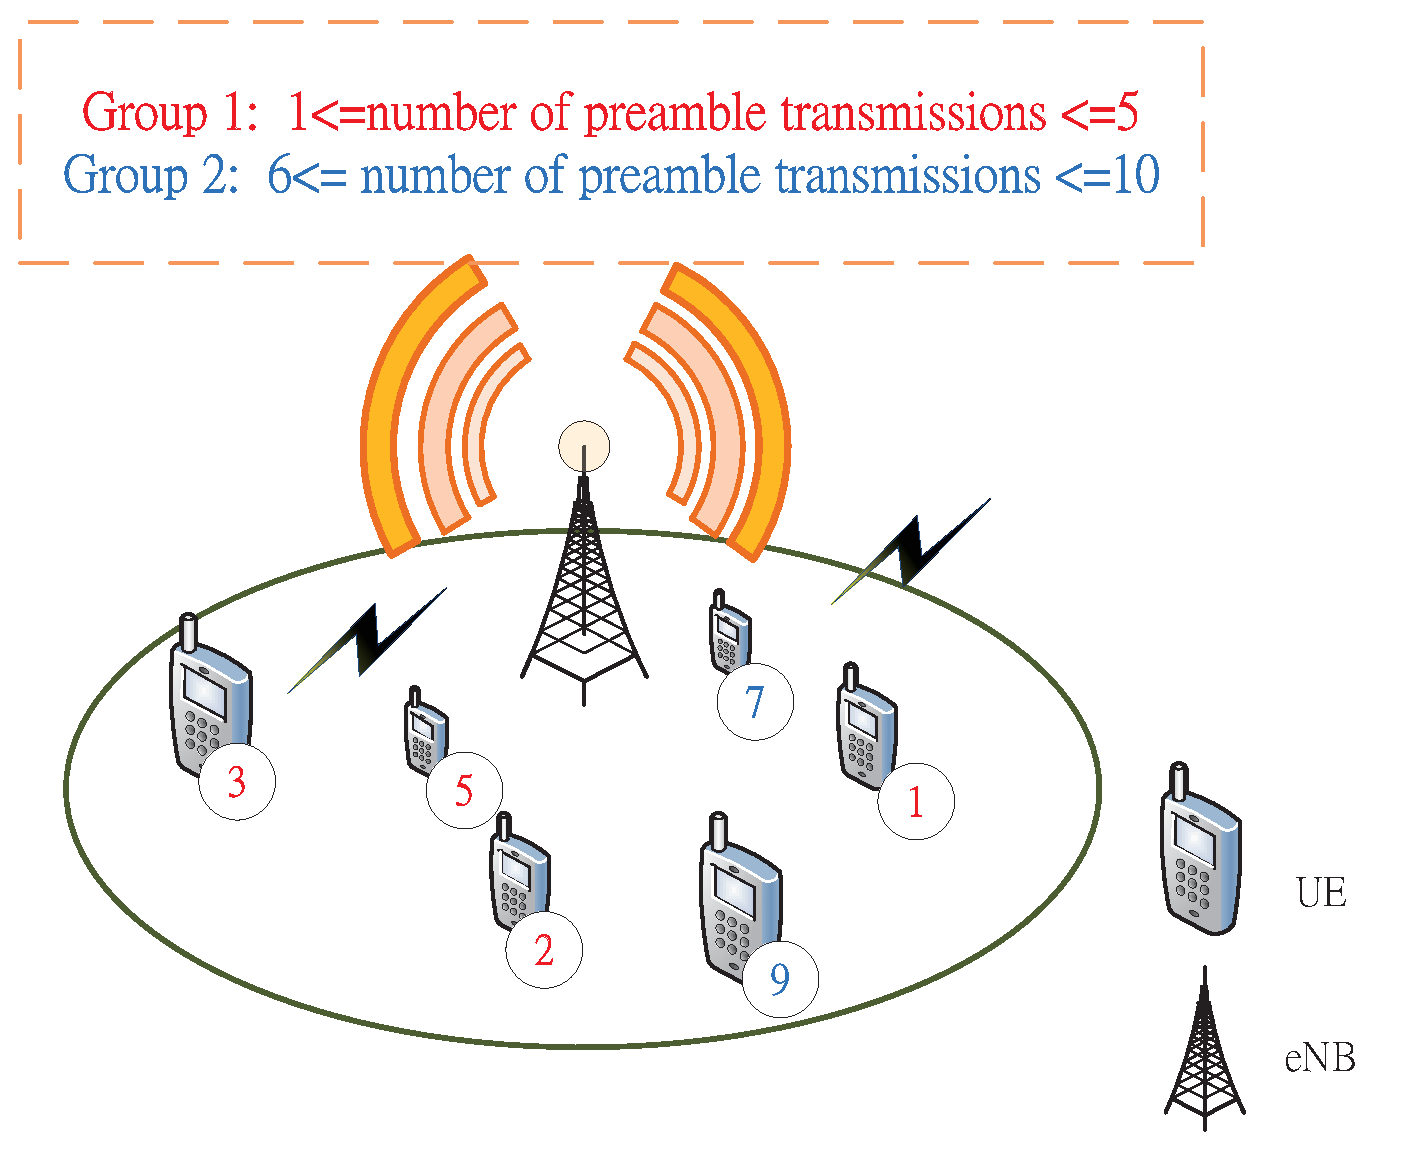
\includegraphics[width=3.8in]{fig_broadcast_groups.eps}
    \caption{Group model of proposed method}
    \label{fig_broadcast_groups}
    \end{figure}
    , MTC devices whose number of preamble transmissions lies in the range between $1$ and $5$ will be classified into group $1$. In the same manner, MTC devices whose number of preamble transmissions lies in the range between $6$ and $10$ will be classified to group $2$.

    Owing to the reason that eNB cannot get the number of devices who try to perform preamble transmission, we aim at obtaining its estimation $N^\prime$ according to the existing information (e.g., number of success preambles and collision preambles). Besides, we let the MTC device who successfully performs preamble transmissions return its number of preamble transmissions when sending the request connection to eNB (in the Msg 3) so that eNB can get the retransmission information of each MTC device from Msg3~\cite{de2015random}. With the retransmission information, eNB is able to calculate $G_{\alpha,\beta}^{m}$, which is the number of devices who belong to $m^{th}$ group and perform $\alpha$th to $\beta$th preamble transmissions in an RACH slot. We can make use of $G_{\alpha,\beta}^{m}$ to observe RAN loading and further change the ACB factor $p$ to cope with different loading condition. Then, we propose an adaptive scheme to change the ACB factor $p$ dynamically. It shows in Fig.~\ref{fig_propose_flow_chart}.
    % \begin{figure}[t]
    % \centering
    % \includegraphics[width=3.8in]{fig_derive.eps}
    % \caption{The block diagram of our proposed retransmission-based ACB scheme}
    % \label{fig_derive}
    % \end{figure}

    \begin{figure}[t]
    \centering
    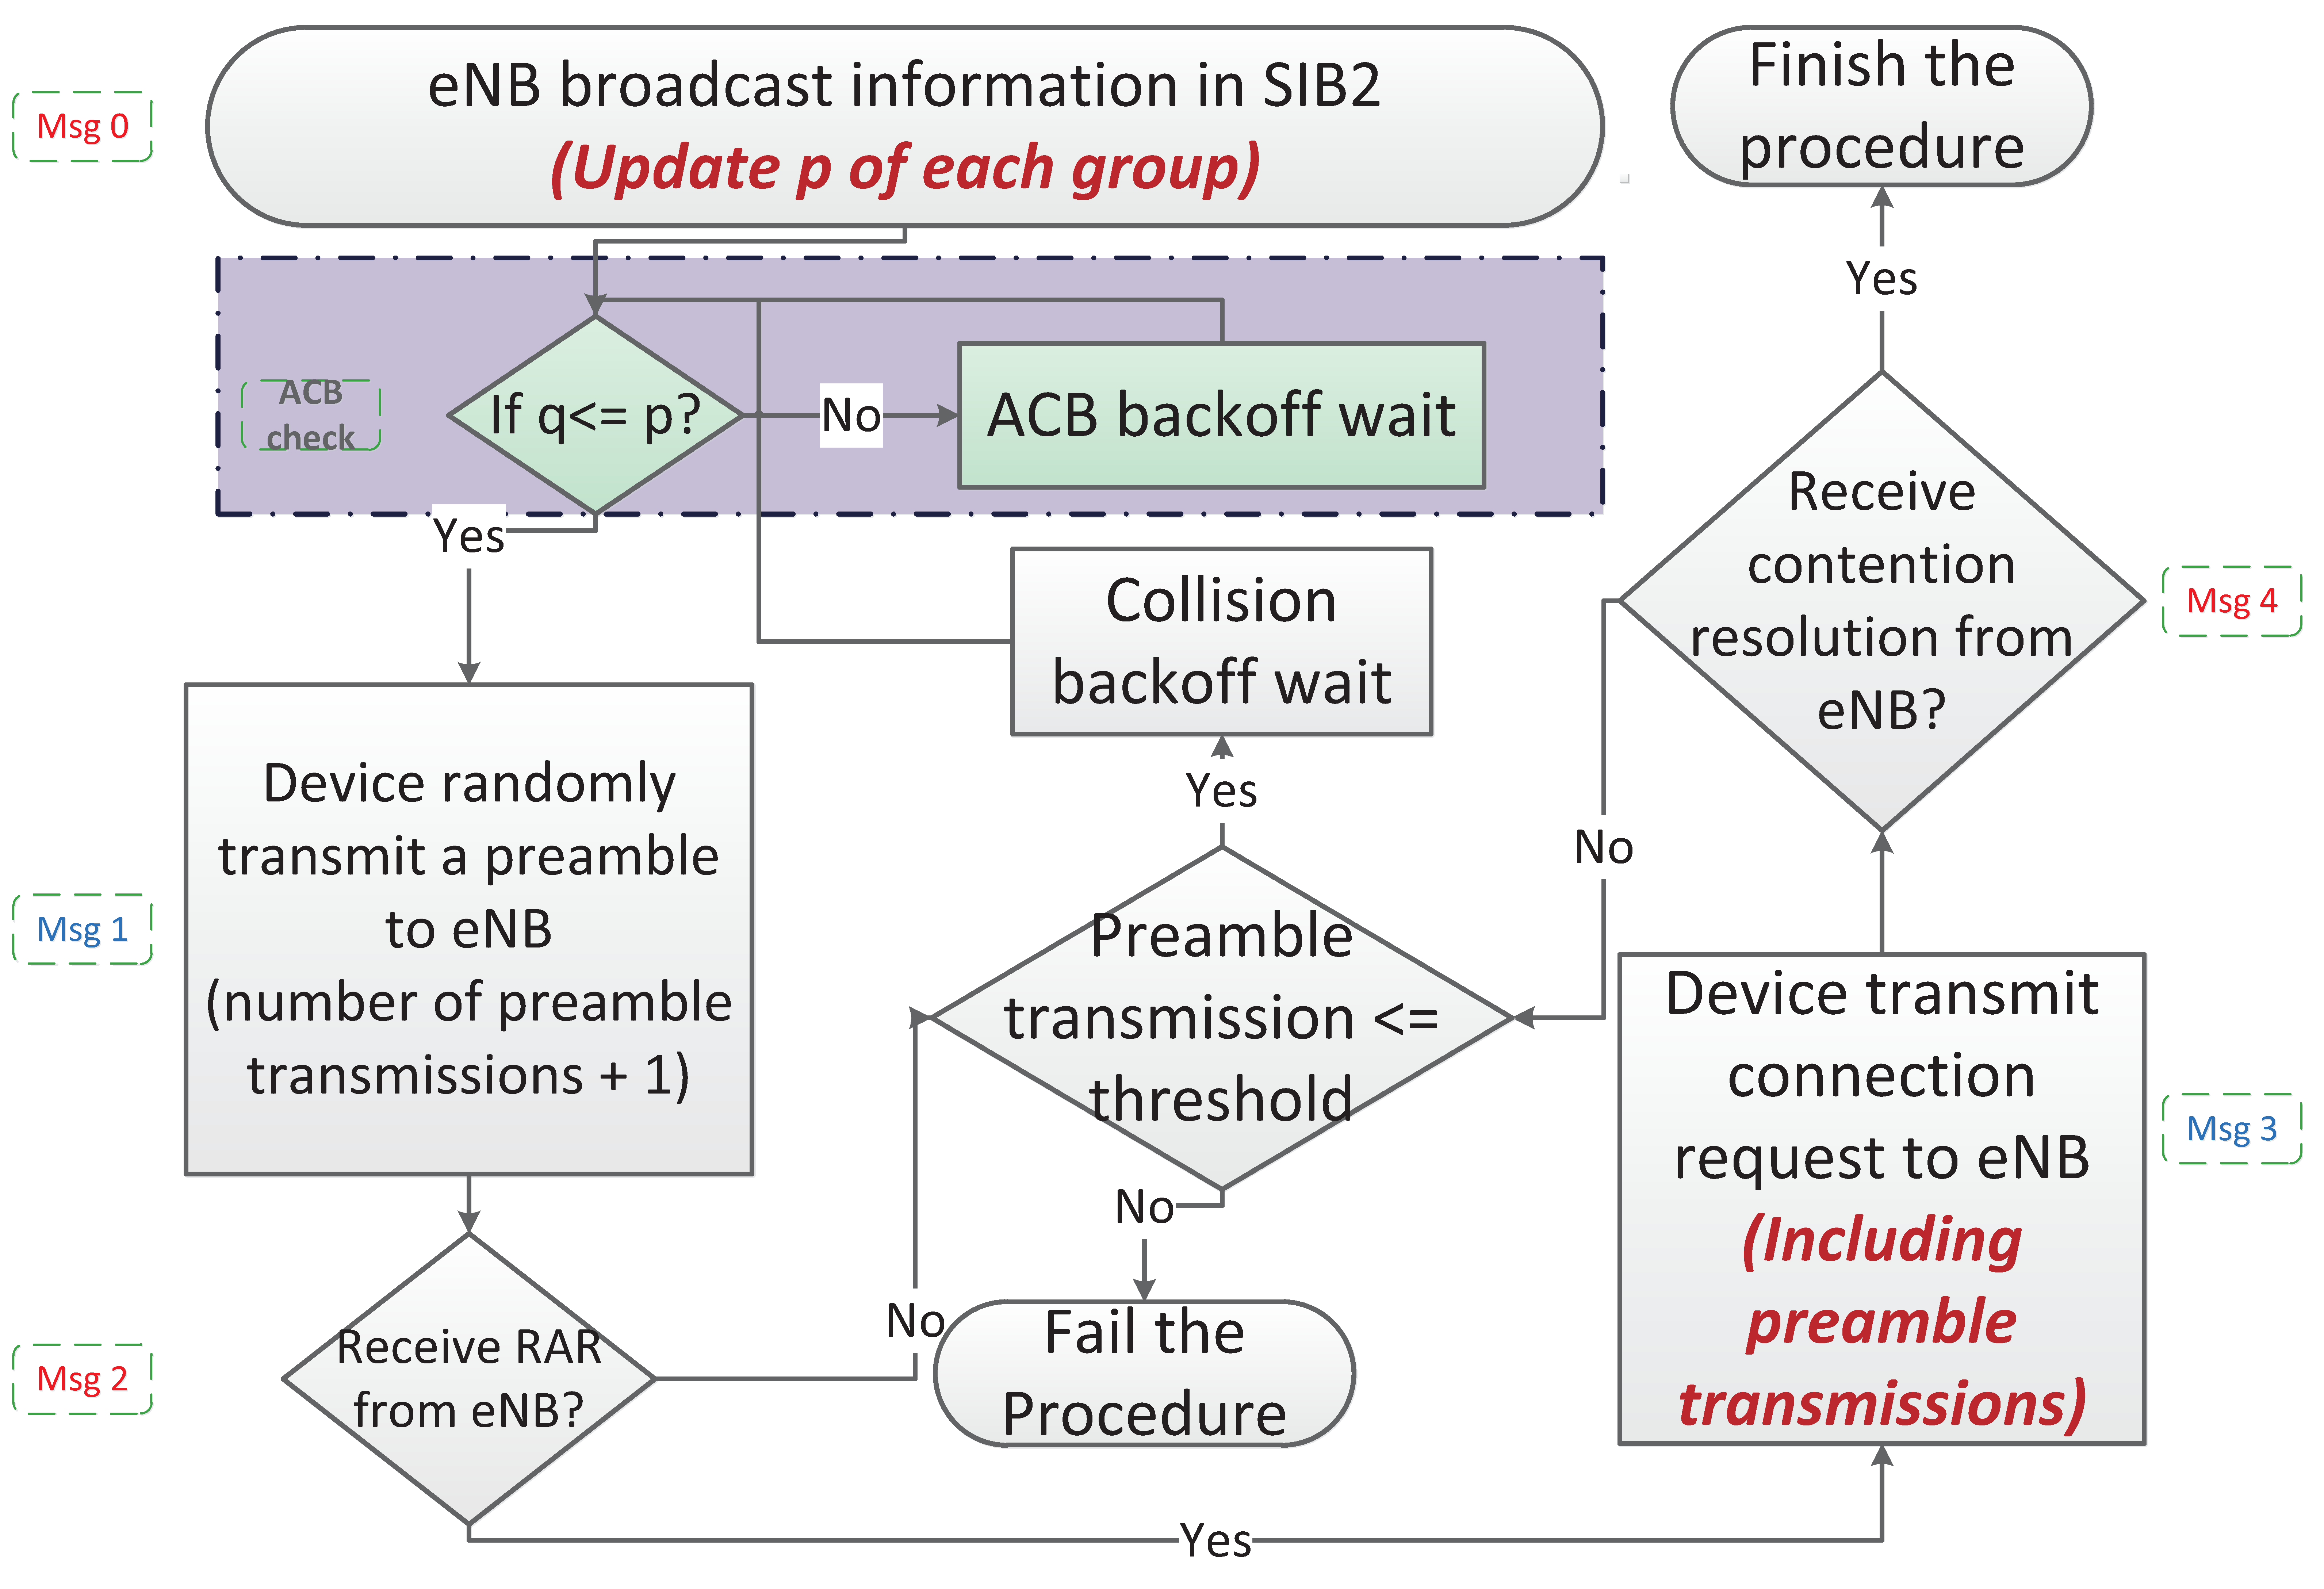
\includegraphics[width=3.8in]{fig_proposed_flow_chart.eps}
    \caption{Retranmission based ACB flow chart}
    \label{fig_propose_flow_chart}
    \end{figure}